\section{Figures}

\begin{figure*}[!ht]
\centering
\includegraphics[width=6in]{figures/map.png}
\caption{Spatial stratification of the Indian Ocean for the four region assessment model (R1a and R1b were treated as one model region but were retained for the fleet definition). The black arrows represent the configuration of the movement parameterization.  Density contours represent of the dispersal of tag releases (red) and subsequent recaptures from Indian Ocean Regional tuna tagging programme. Green circles represent the distribution of catches from the longline fishery aggregated by 5 degree longitude and latitude for 1980 to 2017 (max. = 133 770 t).}
\label{fig:map}
\end{figure*}


\begin{figure*}[!ht]
\centering
\includegraphics[width=6in]{figures/ll.png}
\caption{Regional longline CPUE indices included in the 2018 stock assessment. The difference in scales represents the relative distribtuion of longline vulnearable biomass amongst regions.}
\label{fig:ll}
\end{figure*}

\begin{figure*}[htbp]
\centering
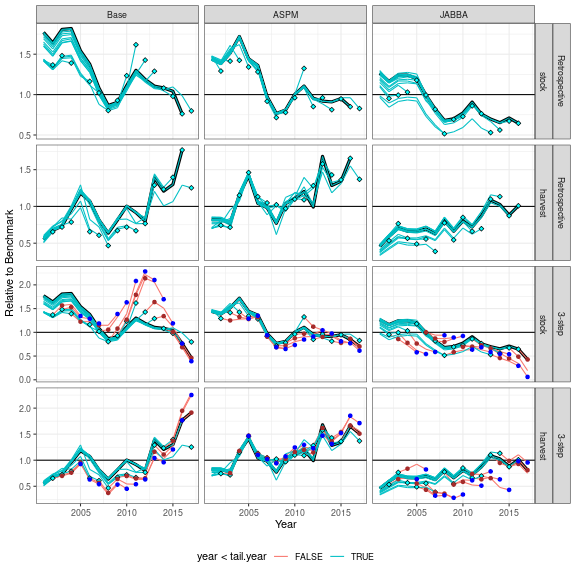
\includegraphics[width=6in]{figures/final-retro-all-1.png}
\caption{Retrospective analysis for the three models, points indicate the terminal years, and the think line the assessment using all the data.}
\label{fig:retro}
\end{figure*}

\begin{figure*}[htbp]
\centering
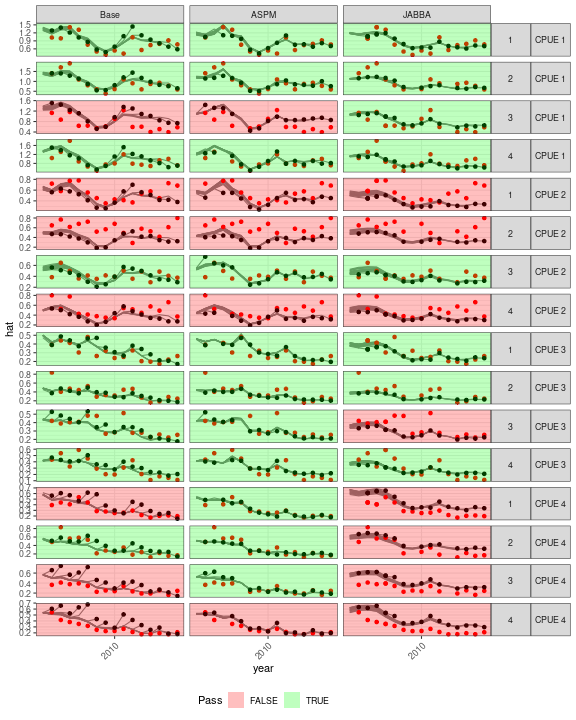
\includegraphics[width=6in]{figures/final-hy-plot-1.png}
\caption{Hindcasts for one step ahead predictions, red dots are the observed CPUE values and lines are the fits with terminal hincast year indicated by a point.}
\label{fig:hy}
\end{figure*}

\begin{figure*}[htbp]
\centering
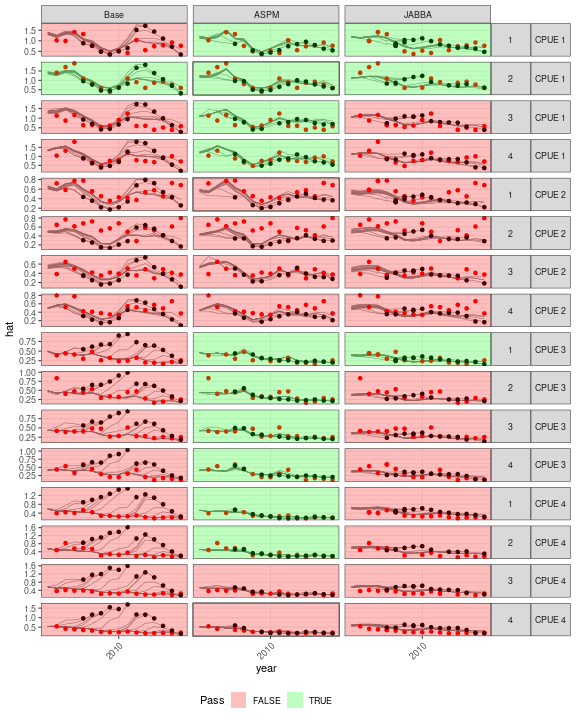
\includegraphics[width=6in]{figures/final-hy3-plot-1.png}
\caption{Hindcasts for three step ahead predictions, red dots are the observed CPUE values and lines are the fits with terminal hincast year indicated by a point.}
\label{fig:hy3}
\end{figure*}

\begin{figure*}[htbp]
\centering
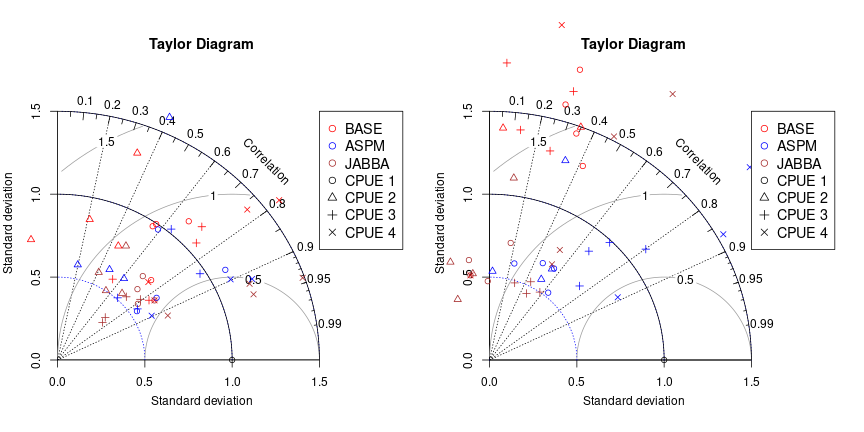
\includegraphics[width=6in]{figures/final-taylor-hy-1-1.png}
\caption{Taylor diagram for one and three year ahead predictions,  summarising the similarity between the observed time series of CPUEs and the predicted relative stock abundance. Each point quantifies how closely predictions match observations, the angle indicates the correlation, the centred root-mean-square error difference between the predicted and observed patterns is proportional to the distance to the point on the x and the contours around this point indicate the RMSE values; the standard deviations of the predictions are proportional to the radial distance from the origin, scaled so the observed pattern has a value of 1. The open circle corresponds to a series which is identical to the reference series. The colours correspond to the model and shape to the survey.)}
\label{fig:td}
\end{figure*}

\begin{figure*}[htbp]
\centering
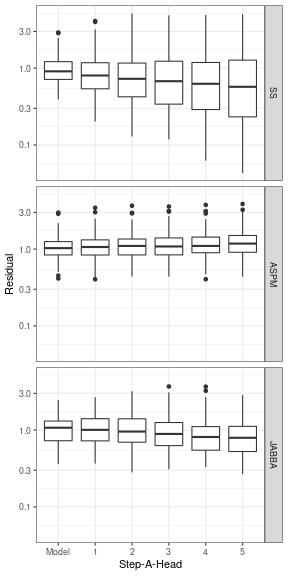
\includegraphics[width=4in]{figures/final-rsdl-1.png}
\caption{Residual for model (Step 0) and predictiion residuals for 1,2,3,4 and 5 steps ahead.}
\label{fig:residuals}
\end{figure*}
